%\documentclass[10pt]{letter}
%\usepackage[utf8]{inputenc}

%%%%%%%%%%%%%%%%%%%%%%%%%%%%%%%%%%%%%%%%%%%%%%%%%
% compile with LuaLatex
%%%%%%%%%%%%%%%%%%%%%%%%%%%%%%%%%%%%%%%%%%%%%%%%%%%%%%%
\documentclass[11pt]{report}
\usepackage{epsfig}
\usepackage{amssymb,amsmath,amsfonts}
\usepackage[activeacute,american]{babel}
%\usepackage[utf8]{inputenc}
\usepackage{subfiles}
\usepackage{cite}
\usepackage{csquotes}
\usepackage{esvect}
\usepackage[acronym,nonumberlist]{glossaries}
\renewcommand{\acronymname}{Nomenclature}
\usepackage{multicol}
\usepackage{caption} 
\usepackage{float}
\usepackage[
    math-style=ISO,      % Upper Case Greek is in italics
    bold-style=ISO,      % Bold math is in italics
    partial=upright,     % nabla and partial upright
    nabla=upright,
  ]{unicode-math}
\topmargin 1.2cm 
\textwidth 16.1cm
\textheight 22.5cm
\oddsidemargin 0.7cm
\setcounter{tocdepth}{5}
\addtolength{\voffset}{-2.4cm}
\addtolength{\hoffset}{-0.5cm}
\usepackage{booktabs}
\usepackage{setspace}
%\doublespacing
\onehalfspacing
\usepackage{caption}
 \captionsetup[figure]{labelfont={bf},name={Figura},labelsep=period}


%%%%%%%%%%%%%%%%%%%%%%%%%%%%%%% 
% citas
% \footnotetext{Mott, Robert L. Mecanica de Fluidos 6/e. Pearson educación, 2006.}
% \footnotetext{Pritchard, Philip J. Fox and McDonald’s Introduction to Fluid Mechanics (8th ed.). John Wiley $\&$ Sons. (2011).}
% \footnotetext{Munson, Bruce R., et al. "Fundamentals of Fluid Mechanics, John Wiley $\&$ Sons." Inc., USA (2006).}
%%%%%%%%%%%%%%%%%%%%%%%%%%%%%%% 

%%%%%%%%%%%%%%%%%%%%%%%%%%%%%%%%%
\begin{document}
\centering{ \textbf{\Large{Mec\'anica de fluidos}}}

\centering {\Large{2$^\circ$ semestre 2020: 541209-1}}
\vspace{1cm}

\flushleft{ \large \underline{\textbf{Pr\'actica 8: Flujos compresibles}}}

%%%%%%%%%%%%%%%%%%%%%%%%%
\vspace{1cm}

\underline {Problema 1:}
\vspace{0.2cm}

Se tiene para una onda de choque estacionaria:
\begin{itemize}
\item $p_1=80$\,kPa
\item $T_1=5$\,$^\circ$C
\item $V_1=600$\,m/s
\end{itemize}
Determine las condiciones de flujo aguas abajo
%%%%%%%%%%%%%%%%%%%%%%%%%
\vspace{0.5cm}

\underline {Problema 2:}
\vspace{0.2cm}

Determine el fluijo m\'asico m\'aximo admisible para la tobera de la figura ~\ref{fig:fig1} y la presi\'on en el plano de salida cuando se tiene flujo estrangulado
\begin{figure}[H]
\centering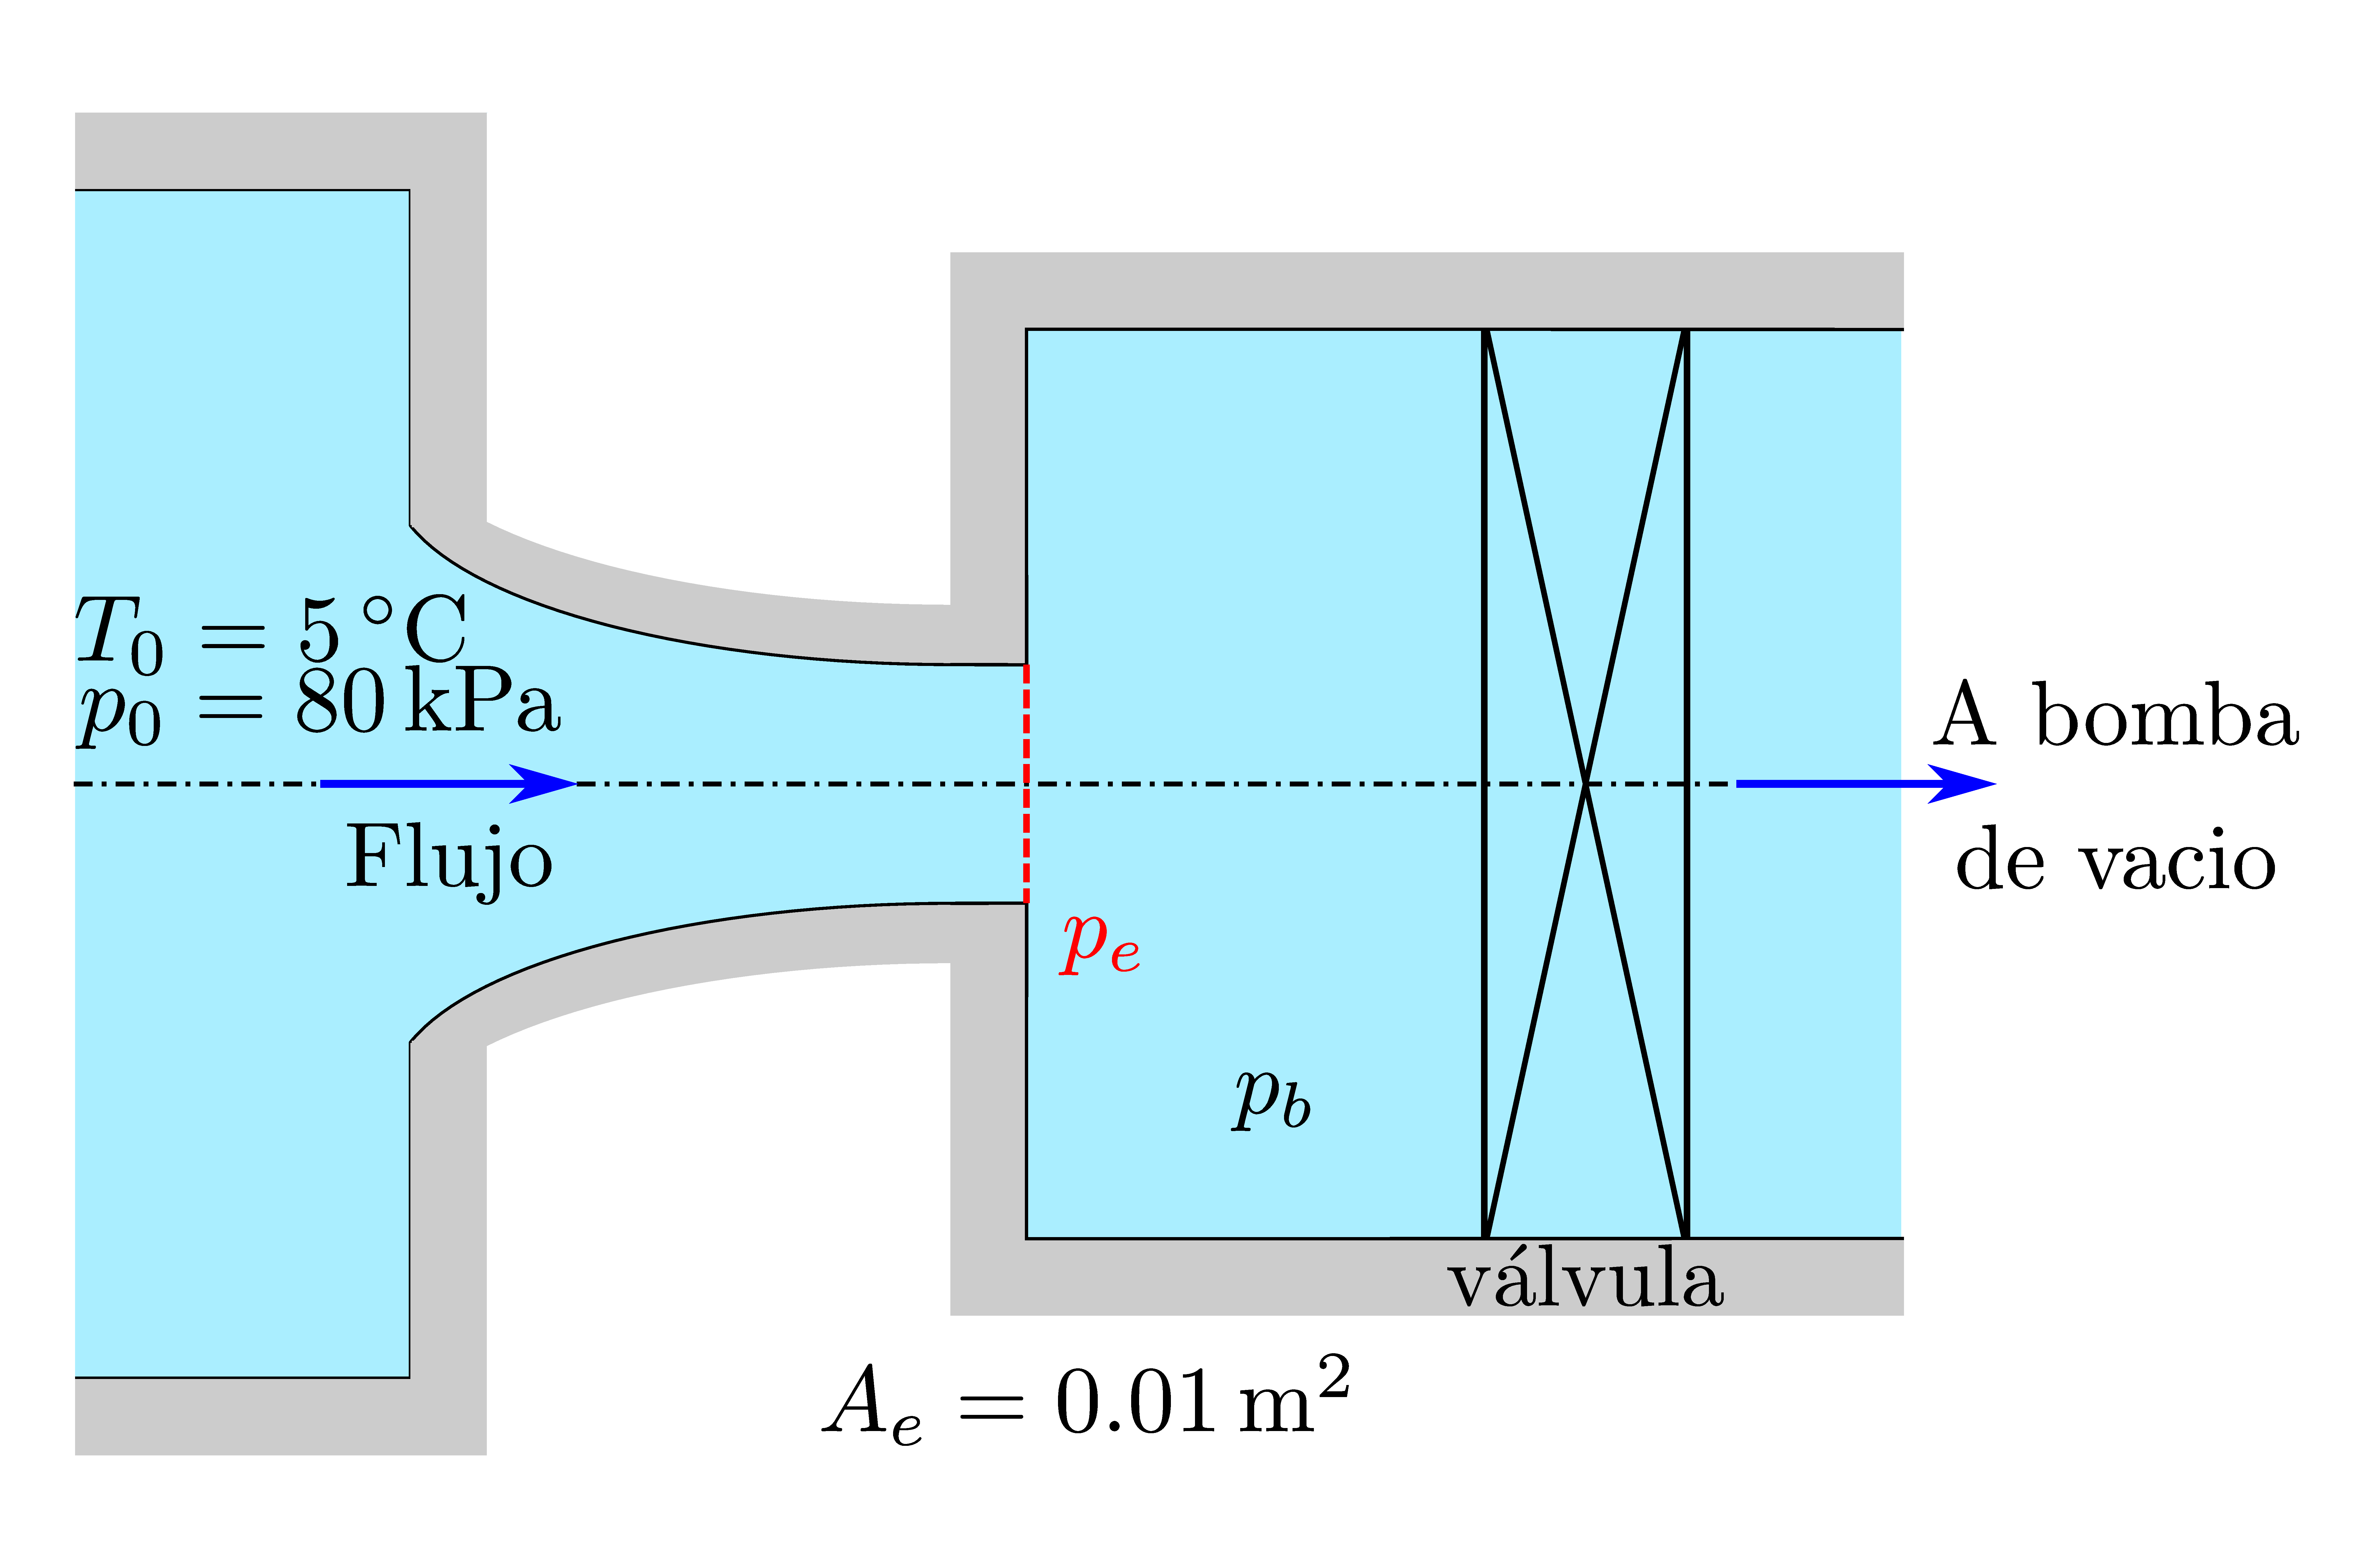
\includegraphics[width=0.8\textwidth]{Figures/tobera_conv.eps}
\caption{\label{fig:fig1} }
\end{figure}

\newpage

\underline {Problema 3:}
\vspace{0.2cm}

Determine las condiciones de flujo en $2$ y $3$ para la tobera representada en la figura~\ref{fig:fig2}. Considere que el flujo es isoentr\'opico en toda la tobera y no se forman ondas de choque.

\begin{figure}[H]
\centering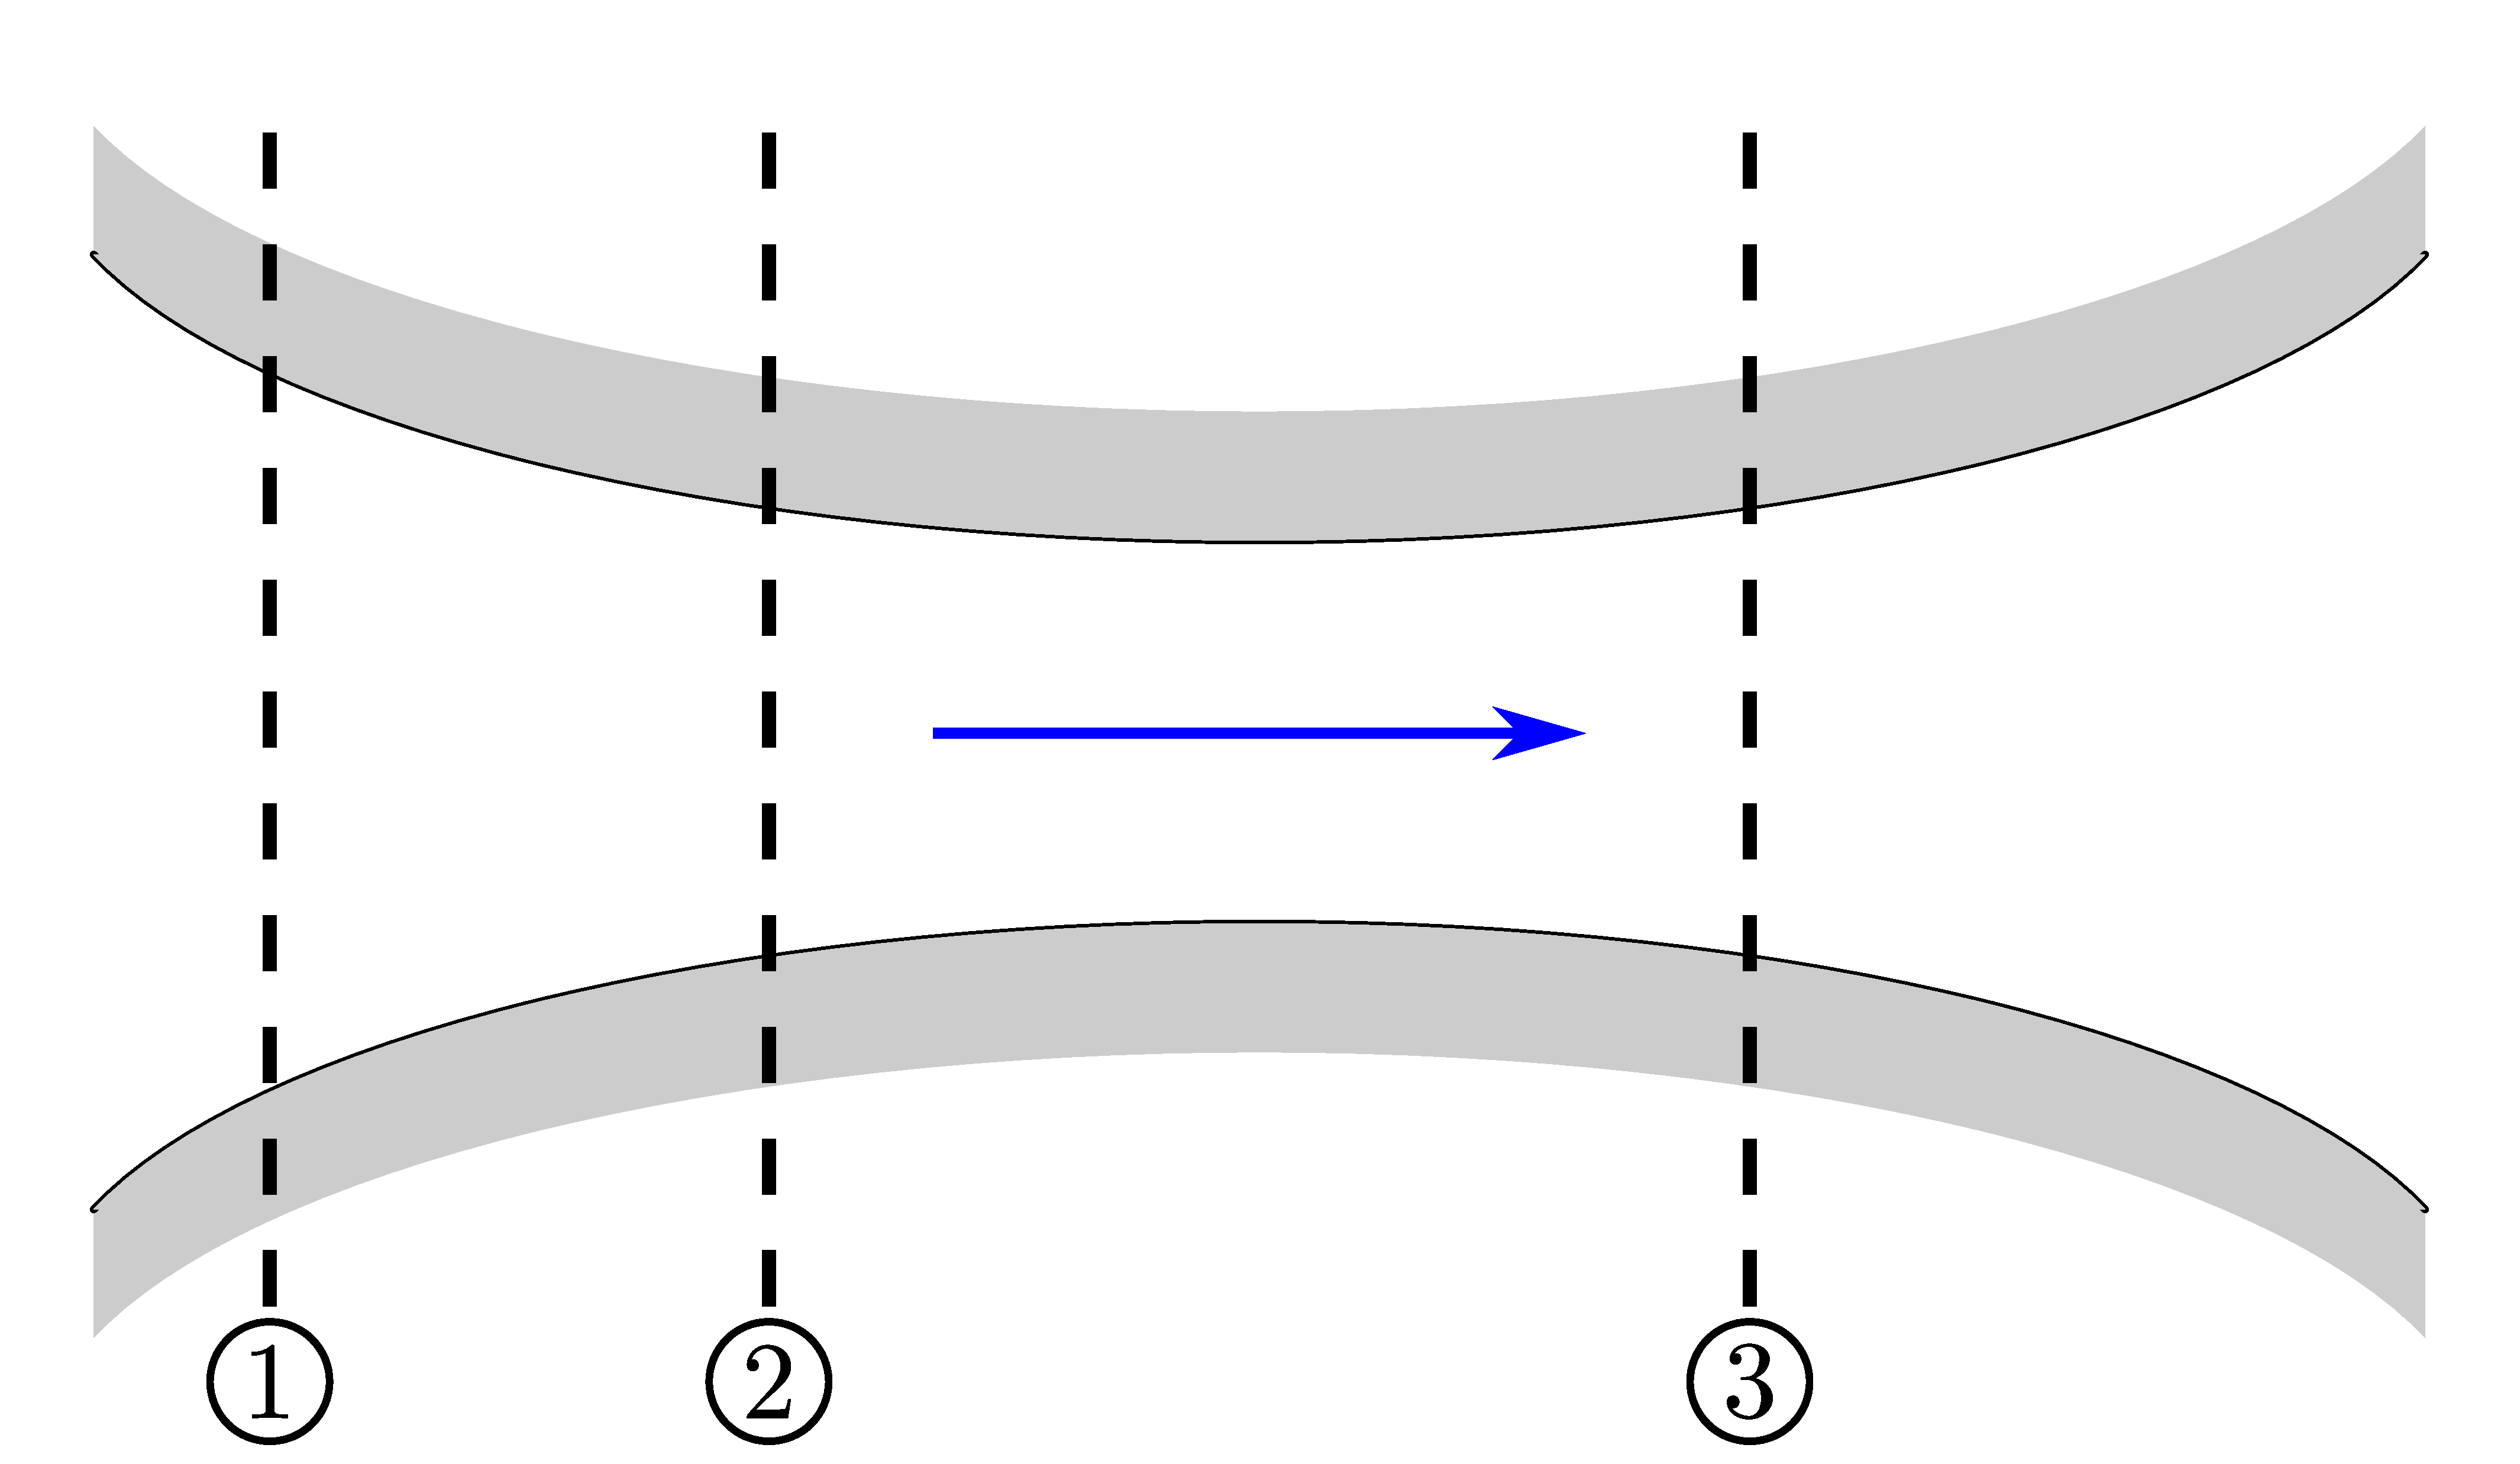
\includegraphics[width=0.5\textwidth]{Figures/conv_div.eps}
\caption{\label{fig:fig2} }
\end{figure}
Considere:
\begin{itemize}
\item $V_1=180$\,m/s
\item $p_1=500$\,kPa
\item $T_1=470$\,K
\item $A_1=0.05$\,m$^2$
\item $A_2=A_3=0.036$\,m$^2$
\item El flujo en $3$ es supers\'onico
\end{itemize}
\vspace{0.2cm}

%%%%%%%%%%%%%%%%%%%%%%%%%
\newpage
\underline {Problema 4:}
\vspace{0.2cm}

Para la tobera presentada en la figura~\ref{fig:fig3} determine:
\begin{enumerate}
\item Condici\'on de diseño
\item Presi\'on m\'axima requerida para que exista flujo supers\'onico en la zona divergente
\item Presi\'on m\'inima requerida para que se formen ondas de choque normales
\item Condiciones de flujo en el plano de salida si $p_b=50$\,kPa. Adem\'as, condiciones de flujo antes y despues de la onda de choque y el \'area transversal de la onda de choque.
\end{enumerate}

\begin{figure}[H]
\centering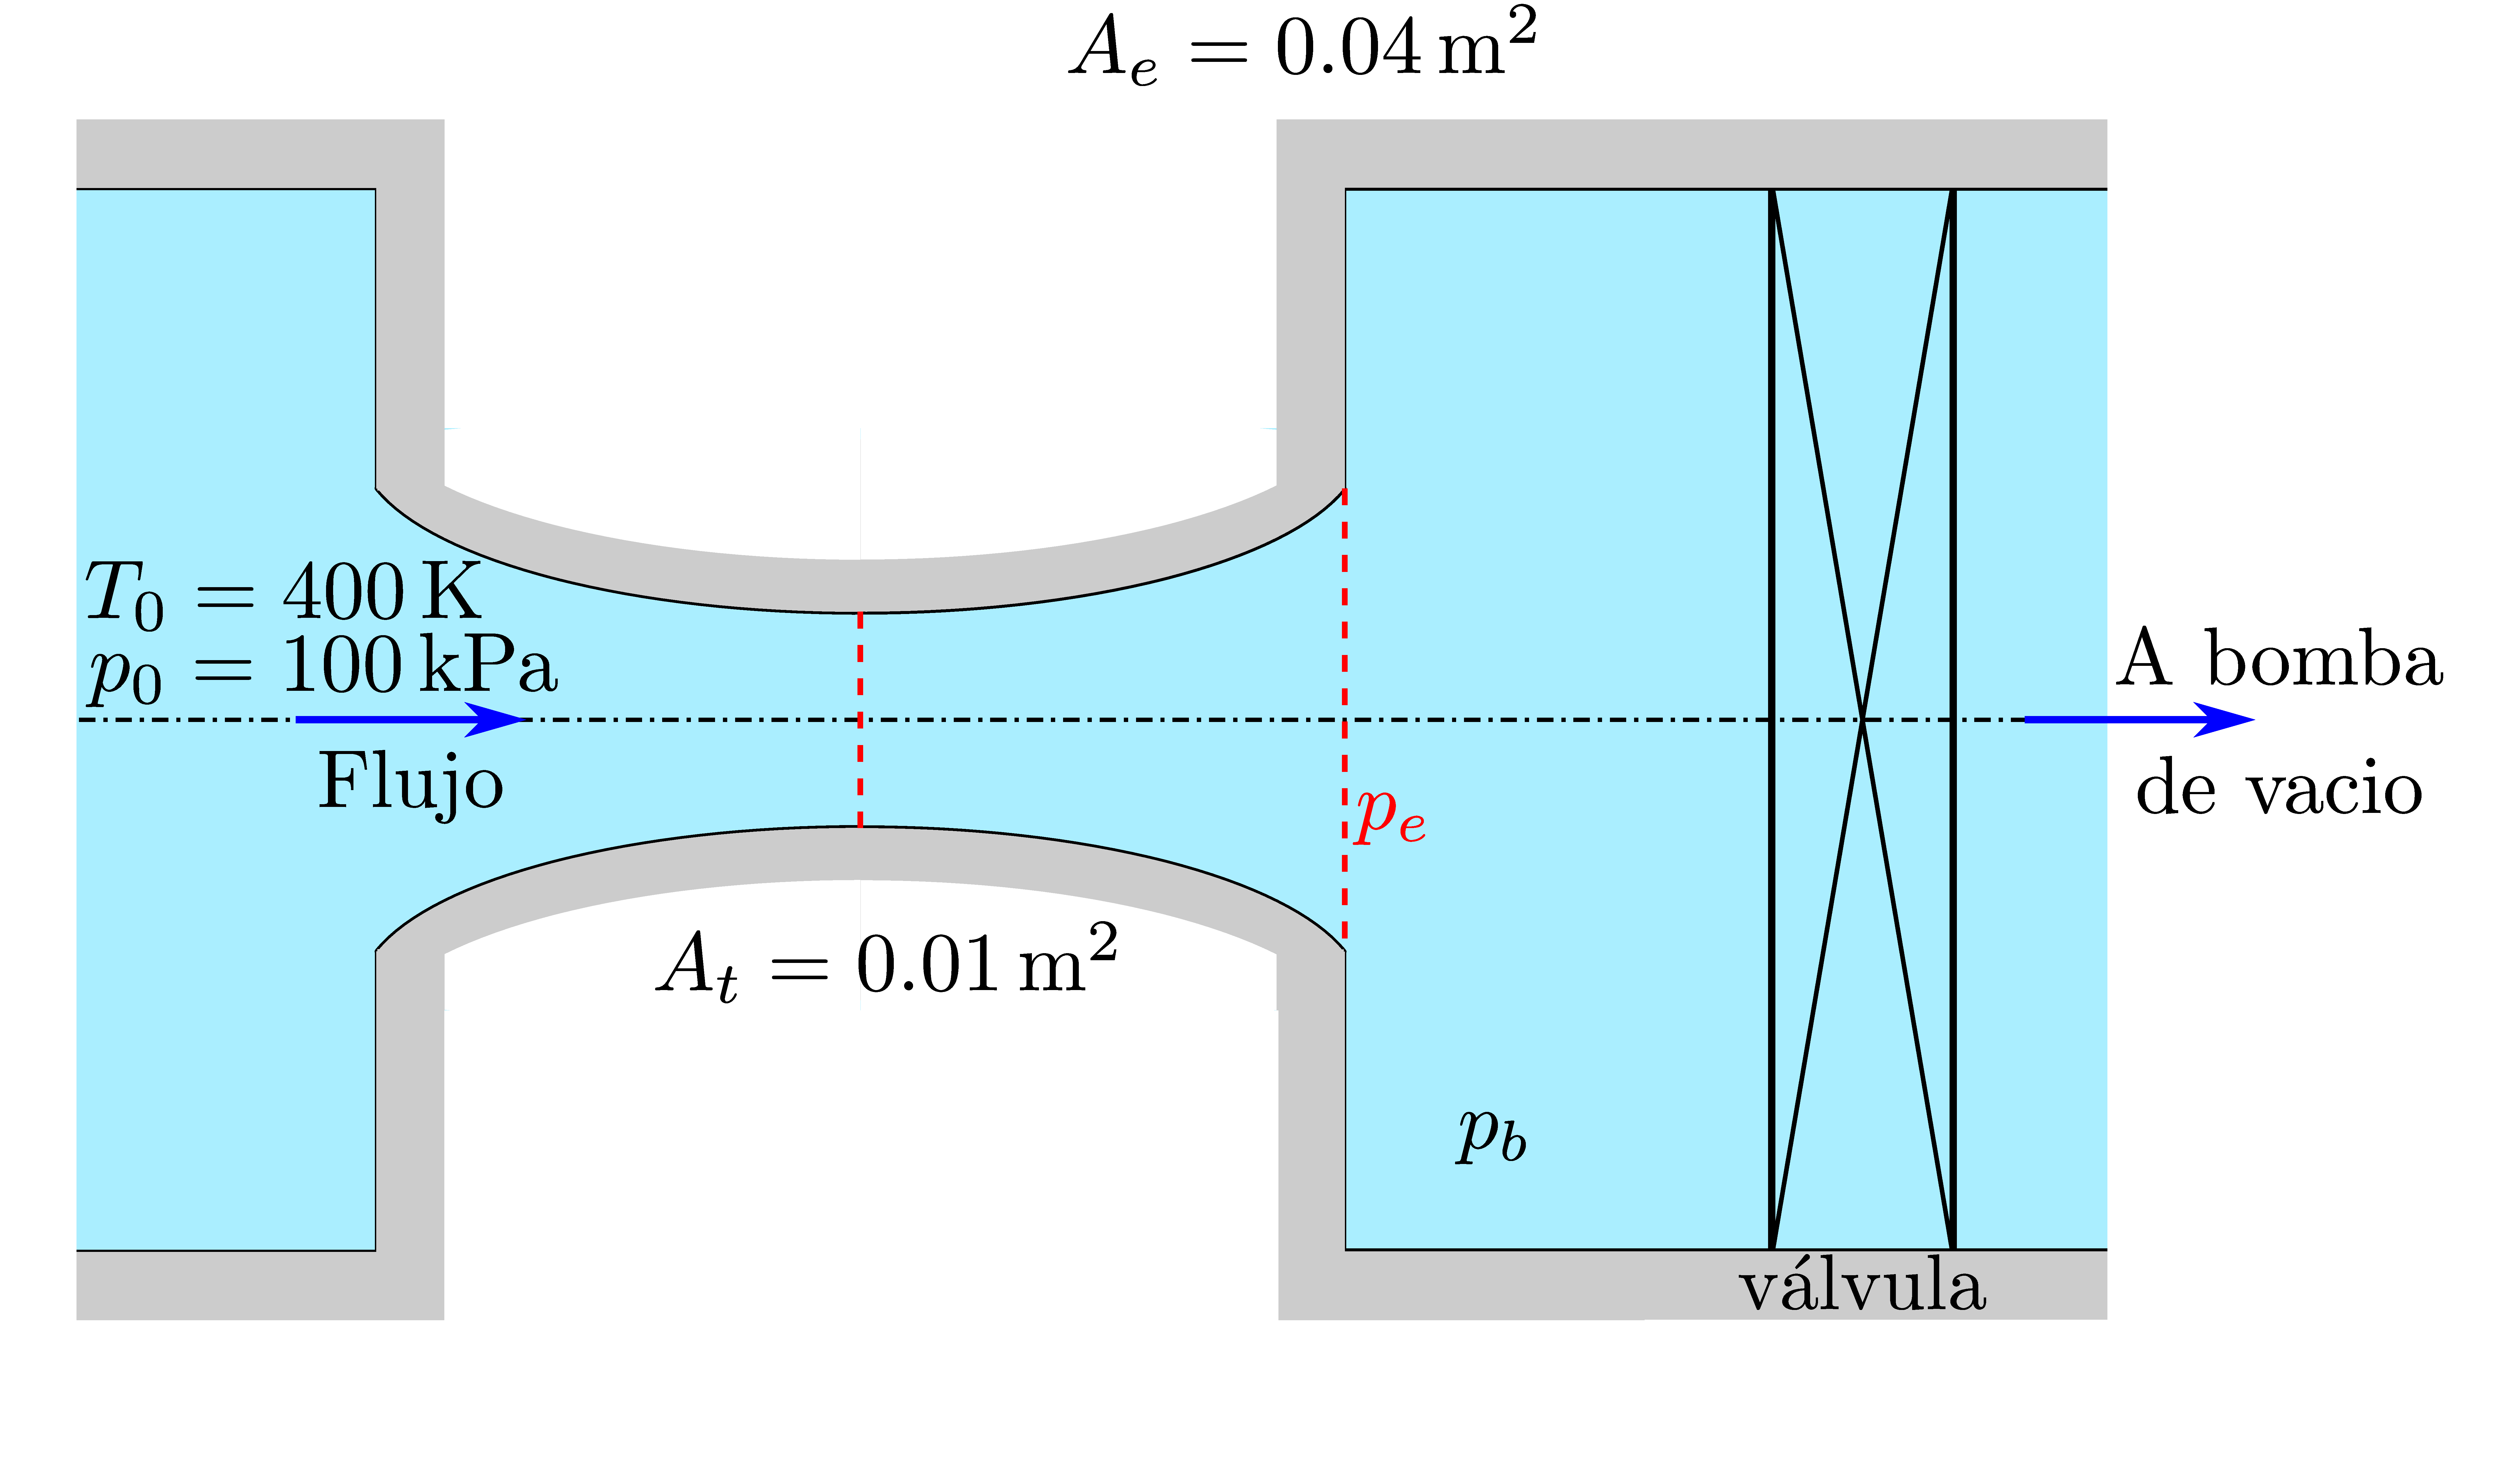
\includegraphics[width=0.8\textwidth]{Figures/tobera_convdiv.eps}
\caption{\label{fig:fig3} }
\end{figure}

%%%%%%%%%%%%%%%%%%%%%%%%%
%%%%%%%%%%%%%%%%%%%%%%%%%
%%%%%%%%%%%%%%%%%%%%%%%%%
\end{document}
